% ---------------------------------------------------------------------------------------------------------------
% TEMPLATE PARA TRABALHO DE CONCLUSÃO DE CURSO
% Instituto Federal de Mato Grosso do Sul - IFMS
% Customização da classe abnTeX2 (http://www.abntex.net.br/) para as normas do IFMS
%
%----------------------------------------------------------------------------------------------------------------
% Codificação: UTF-8
% LaTeX:  abnTeX2          
% ---------------------------------------------------------------------------------------------------------------


% CARREGA CLASSE PERSONALIZADA DO IFMS
\documentclass[
	oneside,			% para impressão em recto e verso.
]{configuracoes/ifms-abntex2}


% INCLUI ARQUIVOS DE CONFIGURAÇÕES
% REFERÊNCIAS------------------------------------------------------------------
\usepackage[%
    alf,
    abnt-emphasize=bf,
    bibjustif,
    recuo=0cm,
    abnt-url-package=url,       % Utiliza o pacote url
    abnt-refinfo=yes,           % Utiliza o estilo bibliográfico abnt-refinfo
    abnt-etal-cite=3,
    abnt-etal-list=3,
    abnt-thesis-year=final
]{abntex2cite}                  % Configura as citações bibliográficas conforme a norma ABNT

% PACOTES----------------------------------------------------------------------
\usepackage[utf8]{inputenc}                                 % Codificação do documento
\usepackage[T1]{fontenc}                                    % Seleção de código de fonte
\usepackage{booktabs}                                       % Réguas horizontais em tabelas
\usepackage{color, colortbl}                                % Controle das cores
\usepackage{float}                                          % Necessário para tabelas/figuras em ambiente multi-colunas
\usepackage{graphicx}                                       % Inclusão de gráficos e figuras
\usepackage{icomma}                                         % Uso de vírgulas em expressões matemáticas
\usepackage{indentfirst}                                    % Indenta o primeiro parágrafo de cada seção
\usepackage{microtype}                                      % Melhora a justificação do documento
\usepackage{multirow, array}                                % Permite tabelas com múltiplas linhas e colunas
\usepackage{subeqnarray}                                    % Permite subnumeração de equações
\usepackage{lastpage}                                       % Para encontrar última página do documento
\usepackage{verbatim}                                       % Permite apresentar texto tal como escrito no documento, ainda que sejam comandos Latex
\usepackage{amsfonts, amssymb, amsmath}                     % Fontes e símbolos matemáticos
\usepackage[algoruled, portuguese]{algorithm2e}             % Permite escrever algoritmos em português
%\usepackage[scaled]{helvet}                                % Usa a fonte Helvetica
\usepackage{times}                                          % Usa a fonte Times
%\usepackage{palatino}                                      % Usa a fonte Palatino
%\usepackage{lmodern}                                       % Usa a fonte Latin Modern
\usepackage[bottom]{footmisc}                               % Mantém as notas de rodapé sempre na mesma posição
\usepackage{ae, aecompl}                                    % Fontes de alta qualidade
\usepackage{latexsym}                                       % Símbolos matemáticos
\usepackage{lscape}                                         % Permite páginas em modo "paisagem"
%\usepackage{picinpar}                                      % Dispor imagens em parágrafos
%\usepackage{scalefnt}                                      % Permite redimensionar tamanho da fonte
%\usepackage{subfig}                                        % Posicionamento de figuras
%\usepackage{upgreek}                                       % Fonte letras gregas
\usepackage{xassoccnt}                                      % Contador de Páginas
\usepackage[scaled]{helvet}
%\usepackage[none]{hyphenat}
\usepackage{xcolor}

%\hyphenchar\font=-1
%\sloppy
%\tolerance=1
%\emergencystretch=\maxdimen
%\hyphenpenalty=10000

% Redefine a fonte para uma fonte similar a Arial (fonte Helvetica)
%\renewcommand{\familydefault}{\sfdefault}
\renewcommand*\familydefault{\sfdefault}


% CONFIGURAÇÕES DE APARÊNCIA DO PDF FINAL--------------------------------------
\definecolor{black}{RGB}{0,0,0}
\makeatletter
\hypersetup{%
    portuguese,
    colorlinks=true,   % true: "links" coloridos; false: "links" em caixas de texto
    linkcolor=black,    % Define cor dos "links" internos
	urlbordercolor=red,
    citecolor=black,    % Define cor dos "links" para as referências bibliográficas
    filecolor=blue,    % Define cor dos "links" para arquivos
    urlcolor=blue,     % Define a cor dos "hiperlinks"
    breaklinks=true,
    pdftitle={\@title},
    pdfauthor={\@author},
    pdfkeywords={abnt, latex, abntex, abntex2}
}
\makeatother

% ALTERA O ASPECTO DA COR AZUL--------------------------------------------------
\definecolor{blue}{RGB}{41,5,195}

% REDEFINIÇÃO DE LABELS---------------------------------------------------------
\renewcommand{\algorithmautorefname}{Algoritmo}
\def\equationautorefname~#1\null{Equa\c c\~ao~(#1)\null}

% CRIA ÍNDICE REMISSIVO---------------------------------------------------------
\makeindex

% HIFENIZAÇÃO DE PALAVRAS QUE NÃO ESTÃO NO DICIONÁRIO---------------------------
\hyphenation{%
    qua-dros-cha-ve
    Kat-sa-gge-los
}




% INSERE CAPA E FOLHA DE ROSTO
% CAPA---------------------------------------------------------------------------------------------------

% ORIENTAÇÕES GERAIS-------------------------------------------------------------------------------------
% Caso algum dos campos não se aplique ao seu trabalho, como por exemplo,
% se não houve coorientador, apenas deixe vazio.
% Exemplos: 
% \coorientador{}
% \departamento{}

% DADOS DO TRABALHO--------------------------------------------------------------------------------------
\titulo{Mundo das Plantas: Catálogo Mobile de Plantas Recorrentes no Pantanal}
\subtitulo{}
\titleabstract{Title in English}
\autor{Angela Egues Barreto\\Patricia da Silva Bandeira}
\autorcitacao{SOBRENOME, Nome} % Sobrenome em maiúsculo
\local{Corumbá}
\data{2019}

% NATUREZA DO TRABALHO-----------------------------------------------------------------------------------
% Opções: 
% - Trabalho de Conclusão de Curso (se for Graduação)
% - Dissertação (se for Mestrado)
% - Tese (se for Doutorado)
% - Projeto de Qualificação (se for Mestrado ou Doutorado)
\projeto{Trabalho de Conclusão de Curso}

% TÍTULO ACADÊMICO---------------------------------------------------------------------------------------
% Opções:
% - Bacharel ou Tecnólogo (Se a natureza for Trabalho de Conclusão de Curso)
% - Mestre (Se a natureza for Dissertação)
% - Doutor (Se a natureza for Tese)
% - Mestre ou Doutor (Se a natureza for Projeto de Qualificação)
\tituloAcademico{Técnico}

% ÁREA DE CONCENTRAÇÃO E LINHA DE PESQUISA---------------------------------------------------------------
% Se a natureza for Trabalho de Conclusão de Curso, deixe ambos os campos vazios
% Se for programa de Pós-graduação, indique a área de concentração e a linha de pesquisa
\areaconcentracao{}
\linhapesquisa{}

% DADOS DA INSTITUIÇÃO-----------------------------------------------------------------------------------
% Se a natureza for Trabalho de Conclusão de Curso, coloque o nome do curso de graduação em "programa"
% Formato para o logo da Instituição: \logoinstituicao{<escala>}{<caminho/nome do arquivo>}
\instituicao{Instituto Federal de Mato Grosso do Sul - IFMS}
\newcommand\instituicaocompleto{Instituto Federal de Educação, Ciência e Tecnologia do Mato Grosso do Sul}
\newcommand\instituicaosigla{IFMS}
\newcommand\instituicaocampus{Campus Corumbá}
%\departamento{}
\programa{Curso Técnico Integrado de Informática}
\newcommand\programanivel{nível Médio}
\logoinstituicao{0.2}{configuracoes/logo_ifms.eps} 

% DADOS DOS ORIENTADORES---------------------------------------------------------------------------------
\orientador{Prof. Vagner da Silva Bezerra}
%\orientador[Orientadora:]{Nome da orientadora}
%\instOrientador{Instituição do orientador}

\coorientador{Prof. M.\textordfeminine Izabelli do Santos Ribeiro}
%\coorientador[Coorientadora:]{Nome da coorientadora}
%\instCoorientador{Instituição do coorientador}

% FOLHA DE ROSTO--------------------------------------------------------------------------------------------------------

% TRABALHO DE CONCLUSÃO DE CURSO
\preambulo{{\imprimirprojeto} apresentado ao {\imprimirprograma} de {\programanivel} do {\instituicaocompleto} - \instituicaosigla, {\instituicaocampus}, em cumprimento às exigências legais como requisito parcial à obtenção do título de {\imprimirtituloAcademico} em Informática.}

%{\imprimirprojeto} apresentado ao Instituto Federal de Mato Grosso do Sul como requisito parcial para a obtenção do título de Técnico de Informática



% DISSERTAÇÃO DE MESTRADO
% \preambulo{{\imprimirprojeto} apresentada ao Programa de \mbox{Pós-graduação} da {\imprimirinstituicao}, como requisito parcial para obtenção do título de {\imprimirtituloAcademico}.}

% TESE DE DOUTORADO
% \preambulo{{\imprimirprojeto} apresentada ao Programa de \mbox{Pós-graduação} da {\imprimirinstituicao}, como requisito parcial para a obtenção do título de {\imprimirtituloAcademico}.}

% PROJETO DE QUALIFICAÇÃO DE MESTRADO OU DOUTORADO
%\preambulo{{\imprimirprojeto} apresentado ao Programa de \mbox{Pós-graduação} da {\imprimirinstituicao}, como requisito parcial para a obtenção do título de {\imprimirtituloAcademico}.}

% OBSERVAÇÕES-----------------------------------------------------------------------------------------------------------
% Altere este arquivo APENAS comentando as linhas que não se aplicam ao tipo de trabalho acadêmico desejado.



% Contagem de Páginas Pré-textuais
\newcounter{realpage}
\DeclareAssociatedCounters{page}{realpage}
\AtBeginDocument{%
	\stepcounter{realpage}
}

\begin{document}

% INSERE ELEMENTOS PRÉ-TEXTUAIS
\pretextual

% Comando para imprimir Capa
\imprimircapa

% Comando para imprimir Folha de rosto
\imprimirfolhaderosto{}                                     		   

% Ficha Catalográfica
% ---
% Inserir a ficha bibliografica
% ---

% Isto é um exemplo de Ficha Catalográfica, ou ``Dados internacionais de
% catalogação-na-publicação''. Você pode utilizar este modelo como referência. 
% Porém, provavelmente a biblioteca da sua universidade lhe fornecerá um PDF
% com a ficha catalográfica definitiva após a defesa do trabalho. Quando estiver
% com o documento, salve-o como PDF no diretório do seu projeto e substitua todo
% o conteúdo de implementação deste arquivo pelo comando abaixo:
%
% \begin{fichacatalografica}
%     \includepdf{fig_ficha_catalografica.pdf}
% \end{fichacatalografica}

\begin{fichacatalografica}
	\sffamily
	\vspace*{\fill}					% Posição vertical
	\begin{center}					% Minipage Centralizado
	\fbox{\begin{minipage}[c][8cm]{13.5cm}		% Largura
	\small
	\imprimirautor
	%Sobrenome, Nome do autor
	
	\hspace{0.5cm} \imprimirtitulo  / \imprimirautor. --
	\imprimirlocal, \imprimirdata
	
	\hspace{0.5cm} \thelastpage p. : il. (algumas color.) ; 30 cm.\\
	
	\hspace{0.5cm} \imprimirorientadorRotulo~\imprimirorientador\\
	\hspace{0.5cm} \imprimircoorientadorRotulo~\imprimircoorientador
	
	\hspace{0.5cm}
	\parbox[t]{\textwidth}{\imprimirtipotrabalho~--~\imprimirinstituicao,
	\imprimirdata.}\\
	
	\hspace{0.5cm}
		1. Palavra-chave1.
		2. Palavra-chave2.
		2. Palavra-chave3.
		I. Orientador.
		II. Universidade xxx.
		III. Faculdade de xxx.
		IV. Título 			
	\end{minipage}}
	\end{center}
\end{fichacatalografica}
% ---

% Folha de Aprovação
% ---

% ---
% Inserir folha de aprovação
% ---

% Isto é um exemplo de Folha de aprovação, elemento obrigatório da NBR
% 14724/2011 (seção 4.2.1.3). Você pode utilizar este modelo até a aprovação
% do trabalho. Após isso, substitua todo o conteúdo deste arquivo por uma
% imagem da página assinada pela banca com o comando abaixo:
%
% \begin{folhadeaprovacao}
% \includepdf{folhadeaprovacao_final.pdf}
% \end{folhadeaprovacao}
%
\begin{folhadeaprovacao}

  \begin{center}
    {\ABNTEXchapterfont\large\imprimirautor}

    \vspace*{\fill}\vspace*{\fill}
    \begin{center}
      \ABNTEXchapterfont\bfseries\Large\imprimirtitulo
    \end{center}
    \vspace*{\fill}
    
    \hspace{.45\textwidth}
    \begin{minipage}{.5\textwidth}
        \imprimirpreambulo
    \end{minipage}%
    \vspace*{\fill}
   \end{center}
        
   Trabalho aprovado. \imprimirlocal, 28 de Junho de 2019:

   \assinatura{\textbf{\imprimirorientador} \\ Orientador} 
   \assinatura{\textbf{\imprimircoorientador} \\ Coorientador} 
   \assinatura{\textbf{Professor} \\ Convidado 1}
   \assinatura{\textbf{Professor} \\ Convidado 2}
   %\assinatura{\textbf{Professor} \\ Convidado 3}
   %\assinatura{\textbf{Professor} \\ Convidado 4}
      
   \begin{center}
    \vspace*{0.5cm}
    {\large\imprimirlocal}
    \par
    {\large\imprimirdata}
    \vspace*{1cm}
  \end{center}
  
\end{folhadeaprovacao}
% ---

% Dedicatória
% DEDICATÓRIA------------------------------------------------------------------

\renewcommand{\dedicatorianame}{DEDICATÓRIA}

\begin{dedicatoria}

Altere este texto inserindo a dedicatória do seu trabalho. 

\end{dedicatoria}


% Agradecimentos
% AGRADECIMENTOS---------------------------------------------------------------

\begin{agradecimentos}[AGRADECIMENTOS]

Edite e coloque aqui os agradecimentos às pessoas e/ou instituições que contribuíram para a realização do trabalho.

É obrigatório o agradecimento às instituições de fomento à pesquisa que financiaram total ou parcialmente o trabalho, inclusive no que diz respeito à concessão de bolsas.

\end{agradecimentos}
        		

% Epígrafe
% EPÍGRAFE---------------------------------------------------------------------

\renewcommand{\epigraphname}{EPÍGRAFE}

\begin{epigrafe}

\textit{Eu denomino meu campo de Gestão do Conhecimento, mas você não pode gerenciar conhecimento. Ninguém pode. O que pode fazer - o que a empresa pode fazer - é gerenciar o ambiente que otimize o conhecimento. (PRUSAK, Laurence, 1997).}

\end{epigrafe}

% OBSERVAÇÕES------------------------------------------------------------------
% Altere o texto para inserir a epígrafe do seu trabalho



% Resumo em Português
% RESUMO--------------------------------------------------------------------------------

\begin{resumo}[RESUMO]
\begin{SingleSpacing}

% Não altere esta seção do texto--------------------------------------------------------
\imprimirautorcitacao. \imprimirtitulo. \imprimirdata. \pageref {LastPage} f. \imprimirprojeto\ – \imprimirprograma, \imprimirinstituicao. \imprimirlocal, \imprimirdata.\\
%---------------------------------------------------------------------------------------

Tendo em vista que há poucas informações disponíveis sobre as diversas espécies de plantas que predominam na região pantaneira, foi pensado em um meio de dispor tais informações a fim de auxiliar em pesquisas futuras e ofertar um conhecimento a mais para a população residente na região.
A disponibilização das informações ocorrerá por meio de uma aplicação mobile em forma de catálogo, fazendo o uso de uma nova tecnologia denominada React Native, pois ela permite a criação de aplicativos híbridos, ou seja, para android e IOS.
Foi escolhido o desenvolvimento de uma aplicação devido a alta utilização de aparelhos celulares nos dias atuais. A mesma  irá conter informações gerais como o nome científico e popular, ocorrência, distribuição geográfica, grau de ameaça,época de floração.
Espera-se, que com o desenvolvimento da aplicação, o  catálogo mobile possa contribuir com a população como uma forma de adquirir mais conhecimentos sobre a flora pantaneira e também auxiliar em pesquisas no ambiente acadêmico.\\


\textbf{Palavras-chave}: Palavra. Segunda Palavra. Outra palavra.

\end{SingleSpacing}
\end{resumo}

% OBSERVAÇÕES---------------------------------------------------------------------------
% Altere o texto inserindo o Resumo do seu trabalho.
% Escolha de 3 a 5 palavras ou termos que descrevam bem o seu trabalho 



% Resumo em Inglês
% ABSTRACT--------------------------------------------------------------------------------

\begin{resumo}[ABSTRACT]
\begin{SingleSpacing}

% Não altere esta seção do texto--------------------------------------------------------
\imprimirautorcitacao. \imprimirtitleabstract. \imprimirdata. \pageref {LastPage} f. \imprimirprojeto\ – \imprimirprograma, \imprimirinstituicao. \imprimirlocal, \imprimirdata.\\
%---------------------------------------------------------------------------------------


\textbf{Keywords}: Word. Second Word. Another word.

\end{SingleSpacing}
\end{resumo}

% OBSERVAÇÕES---------------------------------------------------------------------------
% Altere o texto inserindo o Abstract do seu trabalho.
% Escolha de 3 a 5 palavras ou termos que descrevam bem o seu trabalho 


% Lista de Figuras
% Lista de Figuras----------------------------------------------------------------

\pdfbookmark[0]{\listfigurename}{lof}
\listoffigures*
\cleardoublepage

% OBSERVAÇÕES---------------------------------------------------------------------
% Este arquivo não precisa de ser alterado, pois a lista é gerada automaticamente.


% Lista de Quadros
% LISTA DE QUADROS----------------------------------------------------------------

\renewcommand{\listofquadrosname}{LISTA DE QUADROS}

\pdfbookmark[0]{\listofquadrosname}{loq}
\listofquadros*
\cleardoublepage

% OBSERVAÇÕES---------------------------------------------------------------------
% Este arquivo não necessita de ser editado. A lista é gerada automaticamente.


% Lista de Tabelas
% LISTA DE TABELAS-------------------------------------------------------------

\pdfbookmark[0]{\listtablename}{lot}
\listoftables*
\cleardoublepage

% OBSERVAÇÕES-------------------------------------------------------------------
% Este arquivo não precisa ser alterado, pois a lista é gerada automaticamente.


% Lista de Abreviaturas e Siglas
% LISTA DE ABREVIATURAS E SIGLAS----------------------------------------------------------

%\begin{siglas}
    
%\end{siglas}

% OBSERVAÇÕES-----------------------------------------------------------------------------
% Altere a lista acima para definir os acrônimos e siglas utilizados neste trabalho


% Lista de Símbolos
% LISTA DE SÍMBOLOS------------------------------------------------------------

%\begin{simbolos}
%\end{simbolos}

% OBSERVAÇÕES-------------------------------------------------------------------
% Altere a lista acima para definir os símbolos utilizados no trabalho


% Lista de Algoritmos
% LISTA DE ALGORITMOS----------------------------------------------------------

\newcommand{\algoritmoname}{Algoritmo}
\renewcommand{\listalgorithmcfname}{LISTA DE ALGORITMOS}

\floatname{algocf}{\algoritmoname}
\newlistof{listofalgoritmos}{loa}{\listalgoritmoname}
\newlistentry{algocf}{loa}{0}

\counterwithout{algocf}{chapter}
\renewcommand{\cftalgocfname}{\algoritmoname\space}
\renewcommand*{\cftalgocfaftersnum}{\hfill--\hfill}

\pdfbookmark[0]{\listalgorithmcfname}{loa}
\listofalgorithms
\cleardoublepage

% OBSERVAÇÕES------------------------------------------------------------------
% Este arquivo não precisa ser alterado, pois a lista é gerada automaticamente.


% Sumário
% SUMÁRIO----------------------------------------------------------------------

\renewcommand{\contentsname}{SUMÁRIO}

\pdfbookmark[0]{\contentsname}{toc}
\tableofcontents*
\cleardoublepage


% OBSERVAÇÕES-------------------------------------------------------------------
% Este arquivo não precisa ser alterado, pois o sumário é gerado automaticamente.


% INSERE ELEMENTOS TEXTUAIS
\textual

% Introdução
% INTRODUÇÃO-------------------------------------------------------------------

\chapter{INTRODUÇÃO}
\label{chap:introducao}

O Pantanal é um dos seis biomas brasileiros, ainda que seja o menor é considerado  pouco afetado pelos impactos ambientais em comparação aos demais. Por possuir uma ampla flora, são encontradas inúmeros tipos de espécies diferentes, podendo estas pertencer a mais de um bioma, como o Cerrado, Amazônia, Mata Atlântica e o Chaco Boliviano.

O surgimento do Bioma Pantanal segundo o geólogo \citeonline{ab2006brasil}, ocorreu por meio de abalos tectônicos, o qual causou uma enorme erosão causando o rebaixamento das planícies e levando ao preenchimento detrítico das bacias sedimentares, que ficou denominada como Abóbada. Ao longo do tempo conforme a adaptação e desenvolvimento da vasta Abóbada originou-se o Bioma Pantanal, denominado na época Depressão Pantaneira. 

O Bioma Pantanal é um importante fator a ser estudado, podendo ser fonte de pesquisas acadêmicas e científicas. Porém, são poucos os meios em que são disponibilizados  conteúdos relacionados a flora e fauna do Bioma Pantanal. O presente trabalho tem como objetivo abranger temáticas referente a flora Pantaneira, dos quais foram selecionadas 20 plantas encontradas nesta região, as mesmas foram retiradas do site Web Ambiente e Flora do Brasil 2020, ambas possuem um dos maiores bancos de dados que fornecem informações sobre a flora de todos os biomas brasileiros. 

Tendo definido o objetivo do trabalho,o meio de disponibilizar conteúdos das espécies elegidas, será mediante ao desenvolvimento de uma aplicação mobile híbrida, que seguirá o modelo de um catálogo, o qual disponibilizará informações relevantes sobre a planta, como nome científico, nome popular, área ocupacional, grau de ameaça  e distribuição.

A aplicação tem seu desenvolvimento baseado em uma nova tecnologia, denominada React Native, um framework mobile baseado no React desenvolvido pela empresa Facebook. Este permite o desenvolvimento mobile híbrido, de forma que possa ser utilizado em dispositivos com Sistema Operacional Android e iOS.


% Revisão de Literatura
% REVISÃO DE LITERATURA--------------------------------------------------------

\chapter{REVISÃO DE LITERATURA}
\label{chap:fundamentacaoTeorica}

\section{O Bioma Pantanal}

\subsection{Características}

Este tópico visa conceitualizar características do Bioma Pantanal, tais como o conceito da palavra Bioma, apresentar o comportamento climático do Pantanal juntamente com sua área ocupacional e sua demais caraterísticas.

O termo Bioma, segundo Colinvaux (1993), foi proposto por Shelford, que do grego, Bio significa vida e  Oma, significa massa. No ponto de vista de Font Quer (1953), a mesma definição foi criado pelo pesquisador Clements. O diferencial entre um autor e outro, está relacionado com caracterização da palavra formação e da palavra bioma, visto que antes a formação referia-se apenas à vegetação, e bioma ao conjunto de vegetação com associação da fauna. Agora, nesse novo termo de Font Quer, foi totalmente incluso a fauna. Já no glossário do livro de Clements (1949), encontra-se a definição para bioma: “\textit{Biome- A community of plants and animals, usually of the rank a formation: a biotic community}”. 

O Pantanal é um dos seis biomas brasileiros, considerado um dos mais deslumbrantes e menos afetado pelos impactos ambientais em relação aos demais, o qual ocupa cerca de 25\% da região de Mato Grosso do Sul e 7\% em Mato Grosso, totalizando em aproximadamente 150 mil quilômetros quadrados no Brasil \citeonline{IBGE}, possuindo uma ampla área vegetacional, que por motivos biológicos, encontram-se nele características de outros biomas, como o Cerrado, a Amazônia, a Mata Atlântica e o Chaco boliviano. No verão o clima é quente e com temperatura média em torno de $32\,^{\circ}\mathrm{C}$, no inverno é frio e seco, com média em torno de $21\,^{\circ}\mathrm{C}$ \cite{portal}. A temperatura, o clima e o solo  acabam influenciando no desenvolvimento de algumas espécies de plantas que predominam no Bioma, havendo distribuição da mesma, o qual buscam o ambiente que mais favorece seu desenvolvimento.

\begin{citacao}
	O Pantanal mato-grossense é constituído por um complexo ou mosaico de diferentes biomas florestais de hidro biomas e helô-biomas (carandazais, paratudais), savânicos de piro-peino biomas (cerrados das cordilheiras entre lagoas), florestais de lito biomas (florestas tropicais estacionais caducifólios sobre afloramentos rochosos e solos rasos), campestres de hidro-helô-biomas (campos inundáveis), em meio a rios, lagoas de água doce (baias), lagoas de água salobra e alcalina (salinas) etc., todos pertencentes ao Zonobioma II. \cite{coutinho2006conceito}
\end{citacao}


A região pantaneira apresenta uma vegetação de fácil identificação, ou seja, não é homogênea, tendo a flora diferenciada, de acordo com o solo e a altitude. Podemos analisar  a vegetação do Cerrado, que apresenta árvores de porte médio, entre arbustos e gramíneas. Os capões de mato são encontrados acima das áreas inundáveis e, consequentemente, a paisagem do Pantanal sofre periodicamente mudanças, em épocas de cheia, o rio transborda, alagando campos e morros isolados, formando pequenas ilhas que servem como abrigo para os animais que foram atingidos. Na seca, os rios retomam seus leitos naturais,  revelando os campos conforme a água vai baixando. \cite{eco}

\subsection{Fitogeografia do Pantanal} 

Existem várias teorias que explicam o surgimento do Bioma Pantanal,  este tópico visa apresentar o estudo da distribuição geográfica, dos fatores históricos e biológicos que determinaram o surgimento do Pantanal, por meio de pesquisas realizadas por \citeonline{ab2006brasil} e \citeonline{pott2009vegetaccao}.

Várias teorias surgiram no decorrer do tempo para explicar o surgimento do Pantanal. De acordo com \citeonline[p. ]{ab2006brasil}, geólogo que desenvolveu estudos sobre o espaço brasileiro, as informações obtidas referente a formação do Pantanal demoraram milhares de anos para serem coletadas, passou por processos de pesquisas e análises para obter  uma resposta que esclareça a origem e a evolução do Pantanal.

Uma das teorias, a defendida por \apudonline{ruellan1952escudo}{ab2006brasil}, referência-se a Depressão  do Pantanal como um exemplo de \textit{boutonnière}, uma linguagem geomorfológica francesa, que tem como significado “casa de botão”, o termo refere-se ao Bioma como a casa e as espécies de plantas,os botões. O qual busca identificar muitas estruturas das vegetações que foram modificadas e escavadas ao longo do tempo em terreno Pré-Cambriano, que, por consequências dos processos erosivos, causaram esvaziamento do terreno. Conforme abordado na teoria dos Refúgios e Redutos, o espaço fisiográfico do Pantanal, iniciou-se devido a uma reativação tectônica, o qual causou o rebaixamento das planícies causando um preenchimento detrítico de uma bacia de sedimentação. Ao longo do tempo, por consequências da erosão, originou-se a depressão pantaneira, com o desenvolvimento e adaptação da vasta abóbada regional e de terrenos atingidos \cite{ab2006brasil}. Antes do surgimento da denominação utilizada nos dias atuais, Bioma Pantanal, era considerado apenas como uma vasta abóbada(amontoado de pedras,morros) de escudo, que servia como fornecimento detrítico para as bacias do Grupo Bauru e Parecis.

Na atualidade, o pantanal constitui uma extensa planície de acumulação, com topografia plana e alagada periodicamente, tendo o rio Paraguai e seus afluentes como o principal meio de transporte de água e sedimentos. \cite{souza2006origem}

Segundo pesquisas realizadas por \citeonline{de2010pantanal}, o Pantanal é considerado a maior planície alagada contínua do mundo, possuindo em território brasileiro cerca de 140.000 $km^{2}$,  situado nos estados de Mato Grosso e Mato Grosso do Sul.

O Pantanal tem a vegetação como um dos seus principais fatores atrativos, possuindo cerca de 2.000 espécies de fanerógamas, incluindo 200 exóticas, tendo como as principais famílias: leguminosas e gramíneas. As terrestres herbáceas, aproximadamente 1000 espécies (Pott, 2009).

\begin{citacao}
	A origem da flora do Pantanal vinha sendo atribuída à influência de Cerrado, Amazônia, Mata Atlântica e Chaco, sem o devido levantamento de espécies. Com base em coletas botânicas para herbário e listagem florística, as proporções fitogeográficas são 50\% de espécies de ampla distribuição, 30\% de espécies do Cerrado, e 20\% de outras origens. \cite{pott2009vegetaccao}
\end{citacao}

O Bioma Pantanal possui uma ampla área vegetacional, várias espécies de plantas são encontradas na região, porém, não havia um levantamento de informações para  identificar  quais biomas pertenciam, visto que as mesmas podem ser encontradas em mais de um bioma, tornando-se assim fontes de estudos e pesquisas.		

Os diversos biomas que compõem o Bioma Pantanal estão distribuídos de forma que seja possível obter sua identificação. O Chaco boliviano se localiza ao sudeste do Pantanal, nas sub-regiões de Porto Murtinho e Nabileque, no Estado de Mato Grosso do Sul. O Cerrado predomina na parte leste e a vegetação com características da Amazônia são encontradas juntos aos rios, em partes baixas situado ao Oeste.

\subsubsection{Primeiros Pesquisadores}

O Pantanal por possuir uma rica flora, acabou despertando interesses em alguns pesquisadores europeus, que foram os primeiros a estudarem a vegetação pantaneira. Estudos que demoraram milhares de anos, passando por pesquisas e análises profundas para poder esclarecer a origem e evolução do Bioma.

\begin{citacao}
	As primeiras informações sobre vegetação do Pantanal foram de viagens exploratórias de alguns dos botânicos europeus pioneiros que começaram a desvendar a flora brasileira entre 1825 e 1895. \cite{pott2009vegetaccao}
\end{citacao}

De acordo com \citeonline{salis2006distribuiccao}, a Flora Pantaneira teve suas primeiras informações registrada no final do século XIX por naturalistas europeus, que estudaram espécies de diversas famílias, realizaram levantamentos das espécies ocorrentes no Pantanal e as classificaram de acordo com as regiões em que se desenvolviam de acordo com os aspectos fitossociólogicos.

Estudos realizados por  Ratter et al. (1996, 2003) e Castro et al. (1999), sobre o Cerrado brasileiro, tiveram o intuito de levantar dados sobre os aspectos e distribuições das vegetações encontradas no Pantanal. Diante das observações notou-se um padrão geográfico na distribuição da flora, no qual seis grupos florísticos foram reconhecidos após a comparação e análise de 376 áreas do Cerrado, o grupo do Sudeste, (cerrados do Estado de São Paulo, Paraná e Sul de Minas Gerai); Centro-Sudoeste (cerrados do Distrito Federal e de Minas Gerais); Norte-Nordeste (Bahia, Ceará, Norte de Minas Gerais, Maranhão, Piauí e parte do Leste de Tocantins); Centro-Oeste (Mato Grosso, Mato Grosso do Sul, Goiás , parte do Oeste de Tocantins e Sul do Paraná ); mesotrófico-oeste(cerrados de vários estados, principalmente de Rondônia e Mato Grosso do Sul) e um grupo de áreas disjuntas, formado pelas savanas amazônicas. \cite{souza2006origem}

\section{Vegetações}

Neste tópico serão abordados conteúdos sobre as oito famílias escolhidas para o desenvolvimento deste trabalho, retratando o nome científico, nome popular, época de floração, grau de ameaça, entre outros.

\subsection{Famílias}

As famílias citadas a seguir, possuem  árvores de porte médio e grande. O qual as características das plantas de cada família foram coletadas do site Web Ambiente, o qual contempla o maior banco de dados já produzido no Brasil sobre espécies vegetais nativas além de disponibilizar estratégias para recomposição ambiental.O sistema foi desenvolvido pela EMBRAPA e pela Secretaria de Extrativismo e Desenvolvimento Rural Sustentável - MMA, em cooperação com diversos especialistas de diferentes instituições parceiras.


\section{Sistemas de Catalogação de Espécies}

%Escrever sobre as plataformas de catalogação e fazer suporte em livros e artigos
 
\section{Desenvolvimento Mobile}

Este capítulo tem por objetivo apresentar as categorias de desenvolvimento mobile segundo os pesquisadores \citeonline {da2014paradigmas}, \citeonline{emdesafios} e \citeonline{toledo2016desenvolvimento}.

\begin{citacao}
	“A evolução da tecnologia dos aparelhos celulares permitiu oferecer ao usuário recursos que vão muito além da realização de uma chamada ou do envio de uma mensagem. As melhorias de hardware dos aparelhos celulares permitiram o desenvolvimento de sistemas operacionais mais avançados.”\cite[]{da2014paradigmas}
\end{citacao}

Com o avanço dos Sistemas Operacionais tornou-se factível produzir aplicativos melhores, tornando os aparelhos celulares mais comuns no cotidiano das pessoas devido a comodidade em facilitar a realização de tarefas diárias.

Segundo \citeonline []{emdesafios}, os aplicativos móveis possibilitaram a criação de novos modelos de negócio, em que o usuário pode ter acesso a novos recursos e serviços, por meio de lojas virtuais produzidas por fabricantes de dispositivos móveis. O principal benefício de surgimento de novos modelos é a ligação de serviços e aplicações avançadas de Internet ao aparelho mobile. Entretanto, existem diferentes plataformas tecnológicas para desenvolvimento mobile, incluindo sistemas operacionais e IDE's  (Integrated Development Environment), gerando uma ampla diversidade de soluções disponíveis no mercado. Os aplicativos móveis dependem de uma organização de código específico para que possam ser continuamente executados em diversas plataformas e versões.

\begin{citacao}
	"Limitações de plataforma para distribuição do aplicativo, como, tempo, custo para o desenvolvimento e complexidade das tecnologias necessárias para a sua criação e manutenção são pontos problemáticos em um projeto voltado ao desenvolvimento deste tipo de aplicativo."\cite{emdesafios}
\end{citacao}

Seguindo essa linha de pensamento existem duas maneiras de categorizar
aplicativos, nativas e web, ambos com seus prós e contras. Há também aplicações multiplataformas que englobam algumas funcionalidades de ambas categorias. Pensando nisso é fundamental saber qual utilizar na hora de planejar um desenvolvimento mobile.

\subsection{Desenvolvimento de Aplicações Nativas}

Aplicativos Nativos são aplicações desenvolvidas para determinados SOs, com Linguagens de programação e IDEs específicas. Cada qual com sua responsabilidade, O sistema operacional é responsável por gerenciar os recursos do dispositivo, a linguagem é utilizada na programação do software e o IDE dispõe ferramentas que ajudam na programação da aplicação.

Com a finalidade de melhorar a interação com o usuário, aplicações nativas utilizam recursos presentes no aparelho,como dispositivos de hardware (GPS, microfone, magnetômetro e câmera) e software (e-mails,  calendário, contatos, fotografias e telefone), para isto os aplicativos são instalados diretamente no sistema operacional, facilitando o uso da aplicação no modo off-line, caso não haja acesso a internet.\cite{toledo2016desenvolvimento}

Apesar das múltiplas funcionalidades, aplicativos nativos não são fáceis de desenvolver, pois para ser executado em diversos dispositivos é preciso utilizar uma variedade de plataformas e programar de forma que funcione diversas versões. Devido a grande quantidade de plataformas, mantê-lo atualizado é desvantajoso, pois faz-se necessário uma variedade de teste e distribuição para cada versão.

\subsection{Desenvolvimento de Aplicações Web}

Uma aplicação web móvel nada mais é que um site em formato para celulares, que pode ser acessado de um navegador Web instalado no dispositivo. Tal qual um ambiente web tradicional, é desenvolvido utilizando as linguagens HTML para texto estáticos e imagens, CSS para o design da tela e JavaScript que é responsável pelos efeitos na aplicação. Por serem baseados em navegadores web, as aplicações podem ser executadas em quaisquer dispositivos que possuem acesso a internet.\cite{emdesafios}

Segundo \citeonline {emdesafios}, as aplicações web são mais baratas, de fácil manutenção e não ocupam memória no dispositivo,pois, não precisam ser instaladas, o que as torna vantajosas devido ao fato de serem compatíveis com diversas plataformas.

Mesmo com as diversas vantagens, é necessário o acesso constante à internet em uma velocidade satisfatória para que haja uma rápida troca de dados com os servidores, além de que se o sistema precisar utilizar recursos e funcionalidades do dispositivo as aplicações web podem ser consideradas descartadas.\cite{toledo2016desenvolvimento}.

Como as aplicações nativas, aplicativos web necessitam de vários testes para adequar ao tamanho de tela dos dispositivos e as exigências de cada navegador, uma vez que o mercado de smartphones é amplo e cada fabricante faz uso de navegadores que se adaptam melhor ao seus produtos.

\subsection{Desenvolvimento de Aplicações Híbridas}

As  aplicações híbridas é a junção de aplicativos nativos e WEB, pois como os nativos, aplicações híbridas são baixadas diretamente no dispositivo e fazer uso de funcionalidades e recursos do mesmo, por exemplo a câmera, bluetooth e GPS. Assim com aplicativos WEB, os híbridos fazem uso de linguagens HTML, JavaScript e CSS. \cite{tavares2016introduccao}

A vantagem deste tipo de aplicação é a facilidade no desenvolvimento, pois é preciso apenas um código para ser compilado para diversas plataformas, poupando tempo para o  desenvolvedor, dado que não se faz necessário a programação em várias linguagens.

%\section{Ambientes de Desenvolvimento}
%Neste tópico serão apresentadas as plataformas IDEs que serão utilizadas neste trabalho.

%\subsection{Visual Studio Code}

%O Visual Studio Code, também conhecido como VScode, é uma IDE leve, porém poderoso. Esta possui extensões para diversas linguagens, como PHP e HTML, e dispõe de suporte para JavaScript, TypeScript e Node.js. A IDE possui variadas funcionalidades que auxiliam na produtividade durante o desenvolvimento, por exemplo o conjunto de atalhos de teclado que agiliza o processo de edição do código fonte.\cite{vscode}

%\subsection{MySql Workbench}

%O MySQL Workbench trata-se de uma ferramenta visual unificada para arquitetos de banco de dados, o qual encontra-se disponível para Windows, Linux e Mac OS X. Por meio dele é possível modelar, gerar e gerenciar visualmente banco de dados, pois a ferramenta fornece modelagem de dados de SQL e ferramentas de administração para configuração de servidor, administração de usuários, backup, entre outros paradigmas.


\section{Sistemas Operacionais}

No presente tópico será abordado os conceitos de Sistemas Operacionais, tais como suas funções tecnológicas.

De acordo com \citeonline{toledo2016desenvolvimento}, "São chamados smartphones os telefones celulares que oferecem alta capacidade de processamento", ou seja, oferece recursos avançados e segundo \citeonline []{torres2018biblia}, é um computador que pode ser transportado a palma da mão, e como todo computador os smartphones necessitam de sistemas operacionais para que possam funcionar.

O sistema operacional é responsável por gerenciar processos e realizar a comunicação entre aplicação e hardware, além de disponibilizar ao usuário uma interface, de forma que a utilização fique mais agradável. \cite {velloso2014informatica}

Hoje em dia o mercado de dispositivos móveis oferece numerosos modelos de aparelhos, e cada fabricante opta por um determinado sistema operacional. Para este trabalho foram selecionados dois sistemas operacionais o Android da empresa Google e o iOS da Apple. 

\subsection{Android}

Liderado pela Google, o Android é uma Linguagem Open Source, ou seja, de código livre para dispositivos móveis, como é um projeto Open Source a documentação é pública e livre para todos, o objetivo é evitar qualquer falha no sistema através de feedbacks transmitidos por seus usuários. Dessa maneira o Android torna-se um sistema operacional completo com código-fonte personalizável que pode ser enviado para qualquer dispositivo.

%https://source.android.com/

\subsection{iOS}

Lançado em 2007 junto com o iPhone, o iOS apenas é executado em dispositivos da Apple como iPhone, Apple TV, iPod Touch e iPad. O desenvolvimento nativo de aplicações para iOS é permitido apenas em computadores MAC, devido ao fato de que as ferramentas de desenvolvimento são encontradas apenas nos sistemas da Apple.\cite{garbin2014sistema}

De acordo com \citeonline{leite2017comparativo}, pesquisadores que realizaram um comparativo entre o SO Android e iOS, aplicações da Google são executados normalmente em iOS, o que facilita no desenvolvimento de aplicativos híbridos.

\section{Linguagens de Programação}	

Neste Tópico será apresentado as Linguagens de Programação utilizadas no projeto, bem como sua funcionalidades e benefícios.

\subsection{PHP}

Criada para atender as dificuldades do desenvolvedor e melhorada para as necessidades da sua comunidade, a Linguagem PHP é um esteriótipo do projeto Open Source, desenvolvida por Rasmus Lerdof no ano de 1995.

Segundo \citeonline [p.5]{gilmore2011php}, a linguagem PHP foi criada para fim de praticidade. Lerdof não queria apenas uma linguagem nova no mercado, mas sim, uma solução de prontamente disponível, como resultado foi criada uma linguagem que permite ao usuário, construir aplicações mesmo que com pouco conhecimento.

Os benefícios desta linguagem são a disposição de mais de 180 bibliotecas contendo mais de 1000 funções, a fácil implementação com suporte nativo oferecido por mais de 25 produtos de banco de dados e por ser uma linguagem Open Source é gratuito.


\subsection{JavaScript}

A linguagem JavaScript foi desenvolvida com o objetivo de fornecer interatividade a uma página web. A primeira versão foi lançada em 1995 e implementada em março de 1996 pela Netscape, uma empresa de serviços de computadores do EUA, em parceria com a Sun Microsystems, uma empresa que vendia computadores, componentes e software, que contribuiu para o desenvolvimento de várias tecnologias. A San foi comprada pela Oracle Corporation em 2009,uma empresa de tecnologia multinacional americana.

O básico do JavaScript é definir uma API mínima para trabalhar com textos, arrays, datas e expressões regulares, não incluindo funções de entradas e saídas, como conexão de redes, armazenamento e gráficos. É utilizada pela maioria dos sites e navegadores modernos, incluindo consoles de jogos.\cite{flanagan2004javascript}

\subsection{HTML5 e CSS3}



\section{Frameworks}

De acordo com \citeonline {sawaya2002dicionario}, autora do dicionário de Informática \& Internet, framework é um “conjunto de elementos e suas interligações constituindo a base de um sistema ou projeto”.

Frameworks servem como ponto de partida no desenvolvimento de um projeto, pois reduz o código-fonte reaproveitando métodos, classes e funções presentes no projeto. Além disso, os frameworks fornecem um design padrão e ajustável, para tornar a interface agradável.\cite{gabardo2017laravel}

Segundo \citeonline {gabardo2017laravel}, existem diversos frameworks para quase todas as linguagens, de forma que o desenvolvedor possa escolher a que melhor atende as necessidades do sistema . Para este trabalho foram escolhidas duas Frameworks, para desenvolvimento mobile e web.

\subsection{Ionic}



\subsection{Laravel}

O framework Laravel foi lançado em 2011, foi desenvolvido com o intuito de agilizar a criação de aplicações web. É um framework, que atualmente vem sendo cada vez mais utilizado pelos os programadores, pois um dos principais fatores que o tornam “especial”, é por possuir uma fácil instalação e configuração. 

\begin{citacao}
	Verificou-se os tipos especiais de teste que o framework Laravel fornece, como a parametrização de dados que, além de facilitar o desenvolvimento de software em relação aos relacionamentos do banco de dados, facilita o processo de automação de teste de software.\cite{pelizza2018estudo}
\end{citacao}


O Laravel é baseado na linguagem PHP, e uma de suas desvantagens é a necessidade de requisitos/extensões para um bom funcionamento. Porém, o Laravel possui uma arquitetura MVC (\textit{Model-View-Controller}) e tem como aspecto principal, o de auxiliar no desenvolvimento de aplicações seguras e de alto desempenho de forma ágil e simplificada, com código limpo.\cite{pelizza2018estudo}

%Conectar isso aqui

O composer trata-se de uma ferramenta para gerenciamento de dependências em PHP, permitindo que o desenvolvedor declare as bibliotecas das quais o projeto é dependente, para que assim seja realizado o gerenciamento(instalar/atualizar). \cite{composer}

% Metodologia
% METODOLOGIA------------------------------------------------------------------

\chapter{METODOLOGIA}
\label{chap:metodologia}
Cada capítulo deve conter uma pequena introdução (tipicamente, um ou dois parágrafos) que deve deixar claro o objetivo e o que será discutido no capítulo, bem como a organização do capítulo.

\section{DELINEAMENTO DA PESQUISA}
\label{sec:titSecDelPesq}

Inserir seu texto aqui...

\section{Coleta e Tratamento de Dados com o intuito de testar um título enorme no Sumário do Template latex}
\label{sec:titSecColDad}

Inserir seu texto aqui...

\subsection{Dados Abertos}
\label{sec:titSecColDadAbertos}
Inserir seu texto aqui...

\subsection{Dados Fechados}
\label{sec:titSecColDadFechados}
Inserir seu texto aqui...

% Resultados
% RESULTADOS-------------------------------------------------------------------

\chapter{ANÁLISE E DISCUSSÃO DOS RESULTADOS}

Cada capítulo deve conter uma pequena introdução (tipicamente, um ou dois parágrafos) que deve deixar claro o objetivo e o que será discutido no capítulo, bem como a organização do capítulo.


% Capítulo com Orientações de uso do Template
% ORIENTAÇÕES GERAIS------------------------------------------------------------


% SOBRE AS ILUSTRAÇÕES----------------------------------------------------------
%\chapter{SOBRE AS ILUSTRAÇÕES}
%\label{chap:apSobreIlust}

%A seguir exemplifica-se como inserir ilustrações no corpo do trabalho. As ilustrações serão indexadas automaticamente em suas respectivas listas. A numeração sequencial de figuras, tabelas e equações também ocorre de modo automático.

%Referências cruzadas são obtidas através dos comandos \verb|\label{}| e \verb|\ref{}|. Sendo assim, não é necessário por exemplo, saber que o número de certo capítulo é \ref{chap:fundamentacaoTeorica} para colocar o seu número no texto. Outra forma que pode ser utilizada é esta: \autoref{chap:fundamentacaoTeorica}, facilitando a inserção, remoção e manejo de elementos numerados no texto sem a necessidade de renumerar todos esses elementos.

% FIGURAS-----------------------------------------------------------------------
%\chapter{FIGURAS}
%\label{chap:figuras}

%Exemplo de como inserir uma figura. A \autoref{fig:figura-exemplo1} aparece automaticamente na lista de figuras. Para saber mais sobre o uso de imagens no \LaTeX{} consulte literatura especializada \cite{Goossens2007}.

%Os arquivos das figuras devem ser armazenados no diretório de "/dados".

%\begin{figure}[!htb]
 %   \centering
  %  \caption{Exemplo de Figura}
   % 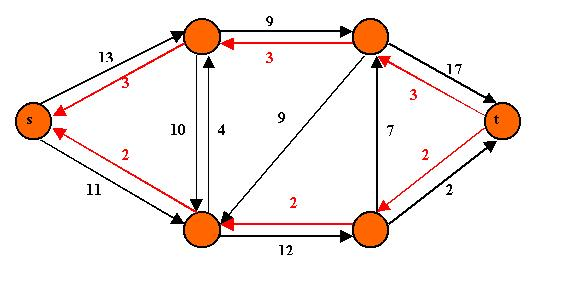
\includegraphics[width=0.5\textwidth]{./dados/figuras/figura1}
    %\fonte{\citeonline{IRL2014}}
    %\label{fig:figura-exemplo1} 
%\end{figure}

% QUADROS E TABELAS---------------------------------------------------------------
%\chapter{QUADROS E TABELAS}
%\label{chap:tabelas}

%Exemplo de como inserir o \autoref{qua:quadro-exemplo1} e a \autoref{tab:tabela-exemplo1}. Ambos aparecem automaticamente nas suas respectivas listas. Para saber mais informações sobre a construção de tabelas no \LaTeX{} consulte literatura especializada \cite{Mittelbach2004}.

%Ambos os elementos (Quadros e Tabelas) devem ser criados em arquivos separados para facilitar manutenção e armazenados no diretório de "/dados".

%\begin{quadro}[!htb]
    \centering
    \caption{Exemplo de Quadro.\label{qua:quadro-exemplo1}}
    \begin{tabular}{|p{7cm}|p{7cm}|}
        \hline
        \textbf{BD Relacionais} & \textbf{BD Orientados a Objetos} \\
        \hline
        Os dados são passivos, ou seja, certas operações limitadas podem ser automaticamente acionadas quando os dados são usados. Os dados são ativos, ou seja, as solicitações fazem com que os objetos executem seus métodos. & Os processos que usam dados mudam constantemente. \\
        \hline
    \end{tabular}
    \fonte{\citeonline{Barbosa2004}}
\end{quadro}


%A diferença entre quadro e tabela está no fato que um quadro é formado por linhas horizontais e verticais. Deve ser utilizado quando o conteúdo é majoritariamente não-numérico. O número do quadro e o título vem acima do quadro, e a fonte, deve vir abaixo. E Uma tabela é formada apenas por linhas verticais. Deve ser utilizada quando o conteúdo é majoritariamente numérico. O número da tabela e o título vem acima da tabela, e a fonte, deve vir abaixo, tal como no quadro.

%\begin{table}[!htb]
    \centering
    \caption[Resultado dos testes]{Resultado dos testes.
    \label{tab:tabela-exemplo1}}
    \begin{tabular}{rrrrr}
        \toprule
            & Valores 1 & Valores 2 & Valores 3 & Valores 4 \\
        \midrule
            Caso 1 & 0,86 & 0,77 & 0,81 & 163 \\
            Caso 2 & 0,19 & 0,74 & 0,25 & 180 \\
            Caso 3 & 1,00 & 1,00 & 1,00 & 170 \\
        \bottomrule
    \end{tabular}
    \fonte{\citeonline{Barbosa2004}}
\end{table}


% EQUAÇÕES-----------------------------------------------------------------------
%\chapter{EQUAÇÕES}
%\label{chap:equacoes}

%Exemplo de como inserir a \autoref{eq:equacao-exemplo1} e a Eq. \ref{eq:equacao-exemplo2} no corpo do texto \footnote{Deve-se atentar ao fato de a formatação das equações ficar muito boa esteticamente.}. Observe que foram utilizadas duas formas distintas para referenciar as equações.

%\begin{equation}
 %   X(s) = \int\limits_{t = -\infty}^{\infty} x(t) \, \text{e}^{-st} \, dt
  %  \label{eq:equacao-exemplo1}
%\end{equation}

%\begin{equation}
    %F(u, v) = \sum_{m = 0}^{M - 1} \sum_{n = 0}^{N - 1} f(m, n) \exp \left[ -j 2 \pi \left( \frac{u m}{M} + \frac{v n}{N} \right) \right]
    %\label{eq:equacao-exemplo2}
%\end{equation}

% ALGORITMOS-----------------------------------------------------------------------
%\chapter{ALGORITMOS}
%\label{chap:algoritmos}

%Exemplo de como inserir um algoritmo. Para inserção de algoritmos utiliza-se o pacote {\ttfamily algorithm2e} que já está devidamente configurado dentro do template.

%Os algoritmos devem ser criados em arquivos separados para facilitar manutenção e armazenados no diretório de "/dados".\\
%\\

%\begin{algorithm}
    \caption{Exemplo de Algoritmo}
    \KwIn{o número $n$ de vértices a remover, grafo original $G(V, E)$}
    \KwOut{grafo reduzido $G'(V,E)$}
    $removidos \leftarrow 0$ \\
    \While {removidos $<$ n } {
        $v \leftarrow$ Random$(1, ..., k) \in V$ \\
            \For {$u \in adjacentes(v)$} {
                remove aresta (u, v)\\
                $removidos \leftarrow removidos + 1$\\
            }
            \If {há  componentes desconectados} {
                remove os componentes desconectados\\
            }
        }
\end{algorithm}


% SOBRE AS LISTAS--------------------------------------------------------------------
%\chapter{SOBRE AS LISTAS}
%\label{chap:apSobreLista}

%Para construir listas de "\textit{bullets}"{} ou listas enumeradas, inclusive listas aninhadas, é utilizado o pacote \verb|paralist|.

%Exemplo de duas listas não numeradas aninhadas, utilizando o comando \verb|\itemize|. Observe a indentação, bem como a mudança automática do tipo de "\textit{bullet}"{} nas listas aninhadas.

%\begin{itemize}
 %   \item item não numerado 1
  %  \item item não numerado 2
   % \begin{itemize}
    %    \item subitem não numerado 1
     %   \item subitem não numerado 2
      %  \item subitem não numerado 3
%    \end{itemize}
 %   \item item não numerado 3
%\end{itemize}

%Exemplo de duas listas numeradas aninhadas, utilizando o comando \verb|\enumerate|. Observe a numeração progressiva e indentação das listas aninhadas.

%\begin{enumerate}
 %   \item item numerado 1
  %  \item item numerado 2
   % \begin{enumerate}
    %    \item subitem numerado 1
     %   \item subitem numerado 2
      %  \item subitem numerado 3
    %\end{enumerate}
    %\item item numerado 3
%\end{enumerate}

% SOBRE AS CITAÇÕES E CHAMADAS DE REFERÊNCAS----------------------------------------------
%\chapter{SOBRE AS CITAÇÕES E CHAMADAS DE REFERÊNCAS}
%\label{chap:apSobreCita}

%Citações são trechos de texto ou informações obtidas de materiais consultadss quando da elaboração do trabalho. São utilizadas no texto com o propósito de esclarecer, completar e embasar as ideias do autor. Todas as publicações consultadas e utilizadas (por meio de citações) devem ser listadas, obrigatoriamente, nas referências bibliográficas, para preservar os direitos autorais. São classificadas em citações indiretas e diretas.

% CITAÇÕES INDIRETAS-----------------------------------------------------------------------
%\chapter{CITAÇÕES INDIRETAS}
%\label{chap:citacoesLivres}

%É a transcrição, com suas próprias palavras, das idéias de um autor, mantendo-se o sentido original. A citação indireta é a maneira que o pesquisador tem de ler, compreender e gerar conhecimento a partir do conhecimento de outros autores. Quanto à chamada da referência, ela pode ser feita de duas maneiras distintas, conforme o nome do(s) autor(es) façam parte do seu texto ou não. Exemplo de chamada fazendo parte do texto:\\
%\\Enquanto \citeonline{Maturana2003} defendem uma epistemologia baseada na biologia. Para os autores, é necessário rever \ldots.\\

%A chamada de referência foi feita com o comando \verb|\citeonline{chave}|, que produzirá a formatação correta.

%A segunda forma de fazer uma chamada de referência deve ser utilizada quando se quer evitar uma interrupção na sequência do texto, o que poderia, eventualmente, prejudicar a leitura. Assim, a citação é feita e imediatamente após a obra referenciada deve ser colocada entre parênteses. Porém, neste caso específico, o nome do autor deve vir em caixa alta, seguido do ano da publicação. Exemplo de chamada não fazendo parte do texto:\\
%\\Há defensores da epistemologia baseada na biologia que argumentam em favor da necessidade de \ldots \cite{Maturana2003}.\\

%Nesse caso a chamada de referência deve ser feita com o comando \verb|\cite{chave}|, que produzirá a formatação correta.

% CITAÇÕES DIRETAS-----------------------------------------------------------------------
%\chapter{CITAÇÕES DIRETAS}
%\label{chap:citacoesLiterais}

%É a transcrição ou cópia de um parágrafo, de uma frase, de parte dela ou de uma expressão, usando exatamente as mesmas palavras adotadas pelo autor do trabalho consultado.

%Quanto à chamada da referência, ela pode ser feita de qualquer das duas maneiras já mencionadas nas citações indiretas, conforme o nome do(s) autor(es) façam parte do texto ou não. Há duas maneiras distintas de se fazer uma citação direta, conforme o trecho citado seja longo ou curto.

%Quando o trecho citado é longo (4 ou mais linhas) deve-se usar um parágrafo específico para a citação, na forma de um texto recuado (4 cm da margem esquerda), com tamanho de letra menor e espaçamento entrelinhas simples. Exemplo de citação longa:
%\\\begin{citacao}
 %   Desse modo, opera-se uma ruptura decisiva entre a reflexividade filosófica, isto é a possibilidade do sujeito de pensar e de refletir, e a objetividade científica. Encontramo-nos num ponto em que o conhecimento científico está sem consciência. Sem consciência moral, sem consciência reflexiva e também subjetiva. Cada vez mais o desenvolvimento extraordinário do conhecimento científico vai tornar menos praticável a própria possibilidade de reflexão do sujeito sobre a sua pesquisa \cite[p.~28]{Silva2000}.
%\end{citacao}

%Para fazer a citação longa deve-se utilizar os seguintes comandos:
%\begin{verbatim}
%\begin{citacao}
%<texto da citacao>
%\end{citacao}
%\end{verbatim}

%No exemplo acima, para a chamada da referência o comando \verb|\cite[p.~28]{Silva2000}| foi utilizado, visto que os nomes dos autores não são parte do trecho citado. É necessário também indicar o número da página da obra citada que contém o trecho citado.

%Quando o trecho citado é curto (3 ou menos linhas) ele deve inserido diretamente no texto entre aspas. Exemplos de citação curta:\\
%\\A epistemologia baseada na biologia parte do princípio de que "assumo que não posso fazer referência a entidades independentes de mim para construir meu explicar" \cite[p.~35]{Maturana2003}.\\
%\\A epistemologia baseada na biologia de \citeonline[p.~35]{Maturana2003} parte do princípio de que "assumo que não posso fazer referência a entidades independentes de mim para construir meu explicar".

% DETALHES SOBRE AS CHAMADAS DE REFERÊNCIAS---------------------------------------------------------
%\chapter{DETALHES SOBRE AS CHAMADAS DE REFERÊNCIAS}
%\label{chap:referUtilizadas}

%Outros exemplos de comandos para as chamadas de referências e o resultado produzido por estes:\\
%\\\citeonline{Maturana2003} \ \ \  \verb|\citeonline{Maturana2003}|\\
%\citeonline{Barbosa2004} \ \ \   \verb|\citeonline{Barbosa2004}|\\
%\cite[p.~28]{Silva2000} \ \ \  \verb|\cite[p.~28]{Silva2000}|\\
%\citeonline[p.~33]{Silva2000} \ \ \   \verb|\citeonline[p.~33]{v}|\\
%\cite[p.~35]{Maturana2003} \ \ \   \verb|\cite[p.~35]{Maturana2003}|\\
%\citeonline[p.~35]{Maturana2003} \ \ \   \verb|\citeonline[p.~35]{Maturana2003}|\\
%\cite{Barbosa2004,Maturana2003} \ \ \   \verb|\cite{Barbosa2004,Maturana2003}|\\

% SOBRE AS REFERÊNCIAS BIBLIOGRÁFICAS-------------------------------------------------------
%\chapter{SOBRE AS REFERÊNCIAS BIBLIOGRÁFICAS}
%\label{chap:apSobreRefer}

%A bibliografia é feita no padrão \textsc{Bib}\TeX{}. As referências são colocadas em um arquivo separado. Neste template as referências são armazenadas no arquivo "base-referencias.bib".

%Existem diversas categorias documentos e materiais componentes da bibliografia. A classe abn\TeX{} define as seguintes categorias (entradas):

%\begin{verbatim}
%@book
%@inbook
%@article
%@phdthesis
%@mastersthesis
%@monography
%@techreport
%@manual
%@proceedings
%@inproceedings
%@journalpart
%@booklet
%@patent
%@unpublished
%@misc
%\end{verbatim}

%Cada categoria (entrada) é formatada pelo pacote \citeonline{abnTeX22014d} de uma forma específica. Algumas entradas foram introduzidas especificamente para atender à norma \citeonline{NBR6023:2002}, são elas: \verb|@monography|, \verb|@journalpart|,\verb|@patent|. As demais entradas são padrão \textsc{Bib}\TeX{}. Para maiores detalhes, refira-se a \citeonline{abnTeX22014d}, \citeonline{abnTeX22014b}, \citeonline{abnTeX22014c}.

% NOTAS DE RODAPÉ--------------------------------------------------------------------------
%\chapter{NOTAS DE RODAPÉ}
%\label{chap:notasRodape}

%As notas de rodapé pode ser classificadas em duas categorias: notas explicativas\footnote{é o tipo mais comum de notas que destacam, explicam e/ou complementam o que foi dito no corpo do texto, como esta nota de rodapé, por exemplo.} e notas de referências. A notas de referências, como o próprio nome ja indica, são utilizadas para colocar referências e/ou chamadas de referências sob certas condições.

        

% Conclusão
% CONCLUSÃO--------------------------------------------------------------------

\chapter{CONCLUSÃO}
\label{chap:conclusao}

Parte final do texto, na qual se apresentam as conclusões do trabalho acadêmico. É importante fazer uma análise crítica do trabalho, destacando os principais resultados e as contribuições do trabalho para a área de pesquisa.

\section{TRABALHOS FUTUROS}
\label{sec:trabalhosFuturos}

Também deve indicar, se possível e/ou conveniente, como o trabalho pode ser estendido ou aprimorado.

\section{CONSIDERAÇÕES FINAIS}
\label{sec:consideracoesFinais}

Encerramento do trabalho acadêmico.


% INSERE ELEMENTOS PÓS-TEXTUAIS
\postextual

% Referências
% REFERÊNCIAS------------------------------------------------------------------

% Carrega o arquivo "base-referencias.bib" e extrai automaticamente as referências citadas


\bibliography{elementos/referencias_bibliograficas}

\bibliographystyle{abntex2-alf} % Define o estilo ABNT para formatar a lista de referências
\renewcommand{\bibname}{\large \MakeUppercase{Referências}}


% OBSERVAÇÕES------------------------------------------------------------------
% Este arquivo não precisa ser alterado.


% Apêndices
% APÊNDICES--------------------------------------------------------------------

\begin{apendicesenv}
\partapendices

% Primeiro apêndice------------------------------------------------------------
\chapter{Nome do apêndice} % Edite para alterar o título deste apêndice
\label{chap:apendiceA}

Lembre-se que a diferença entre apêndice e anexo diz respeito à autoria do texto e/ou material ali colocado.

Caso o material ou texto suplementar ou complementar seja de sua autoria, então ele deverá ser colocado como um apêndice. Porém, caso a autoria seja de terceiros, então o material ou texto deverá ser colocado como anexo.

Caso seja conveniente, podem ser criados outros apêndices para o seu trabalho acadêmico. Basta recortar e colar este trecho neste mesmo documento. Lembre-se de alterar o "label"{} do apêndice.

Não é aconselhável colocar tudo que é complementar em um único apêndice. Organize os apêndices de modo que, em cada um deles, haja um único tipo de conteúdo. Isso facilita a leitura e compreensão para o leitor do trabalho.

% Novo apêndice----------------------------------------------------------------
\chapter{Nome do outro apêndice}
\label{chap:apendiceB}

conteúdo do novo apêndice

\end{apendicesenv}


% Anexos
% ANEXO------------------------------------------------------------------------

\begin{anexosenv}
\partanexos

% Primeiro anexo---------------------------------------------------------------
\chapter{Tabela de Plantas Selecionadas}     % edite para alterar o título deste anexo
\label{chap:anexoA}

\begin{table}[h]
	
	\caption{Relação de Plantas}
	\begin{tabular}{ccccc}
		\hline
		Nome		  	 & Nome Científico 				   			& Família 		& Época de 			 & Grau de			\\
		Popular			 & 											&				& Floração			& Ameaça			\\
		% Note a separação de col. e a quebra de linhas
		\hline                               % para uma linha horizontal
		Acuri   		 & \textit{Attalea phalerata}	   			& Arecaceae 	& ago-jan 			& LC				\\
		& Mart. ex Spreng				   			&				&				    &					\\
		
		Amburana		 & \textit{Amburana cearensis} 	   			& Fabaceae 		& mar-jun 			& NT				\\
		& (Allemão) A.C.Sm				   			&				&				    &					\\
		
		Angico 			 & \textit{Albizia niopoides} 	   			& Fabaceae 		& out-jan 			& LC 				\\
		& (Spruce ex Benth.) Burkart 	   			&				&					&					\\
		
		Aroeira 		 & \textit{Myracrodruon urundeuva} 			& Anacardiaceae	& ago-set 			& LC 				\\
		&  Allemão									&				&				    &					\\
		
		Bocaiúva 		 & \textit{Acrocomia aculeata}      		& Arecaceae 	& out-fev 			& NE 				\\
		&  (Jacq) Lodd. ex Mart.		    		&				&				    &					\\
		
		Cajá 			 & \textit{Spondias mombin}		    		& Anacardiaceae & out-nov 			& NE 				\\
		& L. 						  	    		&				&				    &					\\
		
		Caju 			 & \textit{Anacardium humile}  	    		& Anacardiaceae & ago-nov 			& LC 				\\
		&  A.St.-Hil.					    		&				&			    	&					\\
		
		Caqui do Cerrado & \textit{Diospyros hispida}  	    		& Ebenaceae 	& ago-nov 			& LC 				\\
		&  A.DC						    		&				&				   	&					\\
		
		Caranda 		 & \textit{Copernicia alba}  	    		& Arecaceae 	& jul-dez 			& NE 				\\
		& Morong ex Morong \& Britton	    		&				&					&					\\
		
		Gonçalo 		 & \textit{Astronium fraxinifolium}			& Anacardiaceae & jul-set 			& LC 				\\
		&  Schott.									&				&				    &					\\
		
		Ipê-Amarelo		 & \textit{Tabebuia aurea}   				& Bignoniaceae 	& ago-out 			& NE 				\\
		& (Silva Manso) Benth. \&	Hook.f.			&				&				    &					\\
		& ex S.Moore								&				&				    &					\\
		
		Ipê-Branco 		 & \textit{Tabebuia roseoalba}  			& Bignoniaceae 	& ago-dez			& NE 				\\
		& (Ridl.) Sandwith 						&				&				    &					\\
		
		Ipê-Verde 		 & \textit{Cybistax antisyphilitica}		& Bignoniaceae  & ago-mar 			& NE 				\\
		& (Mart) Mart 								&				&				    &					\\
		
		Jenipapo 		 & \textit{Genipa americana}  				& Rubiaceae 	& set-dez 			& LC 				\\
		& L. 										&				&				    &					\\
		
		Louro Preto 	 & \textit{Cordia glabrata}  				& Boraginaceae 	& ago-out 			& NE 				\\
		& (Mart.) A.DC. 							&				&				    &					\\
		
		Passarinho 		 & \textit{Pterogyne nitens}  				& Fabaceae 		& fev-ago 			& LC 				\\
		& Tul										&				&				    &					\\
		
		Pata de vaca 	 & \textit{Bauhinia rufa}	  				& Fabaceae 		& mai-nov 			& NE 				\\
		&  (Bong.) Steud.							&				&				    &					\\
		
		Sucupira 		 & \textit{Bowdichia virgilioides}		  	& Fabaceae 		& jun-ago 			& NT 				\\
		& Kunth									&				&				    &					\\
		
		Tarumã           & \textit{Vitex cymosa}	 				& Lamiaceae 	& set-nov 			& NE 				\\
		&  Bertero ex Spreng.						& 				&					&					\\
		
		Ximbuva 		 & \textit{Enterolobium contortisiliquum}	& Fabaceae 		& set-nov 			& NE 				\\
		&  (Vell.) Morong 							&				&					&					\\
		\hline
	\end{tabular}
\end{table}
% Novo anexo-------------------------------------------------------------------
\chapter{Nome do outro anexo}
\label{chap:anexoB}

conteúdo do outro anexo

\end{anexosenv}


\end{document}
